% ============================================================================
% TRM vs TRC - Adaptation Diagram
% ============================================================================
% Shows how TRC adapts TRM for control problems
% Compile with: pdflatex paper_figure_trm_vs_trc.tex
% ============================================================================

\documentclass[tikz,border=5pt]{standalone}
\usepackage{tikz}
\usepackage{amsmath}
\usetikzlibrary{shapes.geometric, arrows.meta, positioning, calc, backgrounds, decorations.pathreplacing}

% Define colors
\definecolor{trmcolor}{RGB}{100, 100, 100}
\definecolor{trccolor}{RGB}{52, 168, 83}
\definecolor{novelcolor}{RGB}{255, 87, 34}
\definecolor{sharedcolor}{RGB}{66, 133, 244}

\begin{document}

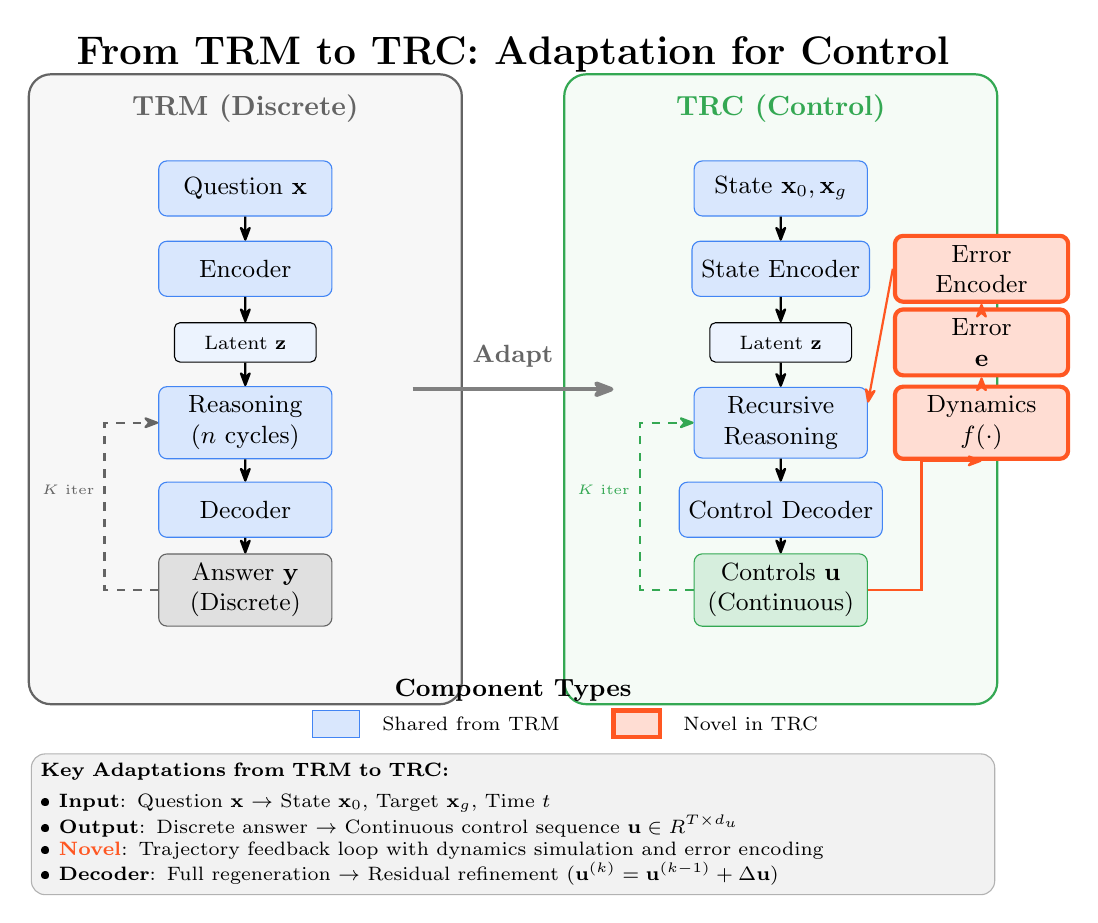
\begin{tikzpicture}[
    scale=0.85,
    >={Stealth[round]},
    box/.style={rectangle, rounded corners=3pt, draw, minimum width=2.2cm, minimum height=0.7cm, align=center, font=\small},
    smallbox/.style={rectangle, rounded corners=2pt, draw, minimum width=1.8cm, minimum height=0.5cm, align=center, font=\scriptsize},
    arrow/.style={->, thick},
    label/.style={font=\footnotesize}
]

% Title
\node[font=\Large\bfseries] at (6.5, 7) {From TRM to TRC: Adaptation for Control};

% ===================== LEFT: TRM (Original) =====================
\begin{scope}[on background layer]
\node[draw=trmcolor, thick, rounded corners=8pt, fill=trmcolor!5,
      minimum width=5.5cm, minimum height=8cm] at (2.5, 2) {};
\end{scope}
\node[font=\bfseries, text=trmcolor] at (2.5, 6.2) {TRM (Discrete)};

% TRM components
\node[box, fill=sharedcolor!20, draw=sharedcolor] (trm_x) at (2.5, 5) {Question $\mathbf{x}$};
\node[box, fill=sharedcolor!20, draw=sharedcolor] (trm_enc) at (2.5, 3.8) {Encoder};
\node[smallbox, fill=sharedcolor!10] (trm_z) at (2.5, 2.7) {Latent $\mathbf{z}$};
\node[box, fill=sharedcolor!20, draw=sharedcolor] (trm_reason) at (2.5, 1.5) {Reasoning\\($n$ cycles)};
\node[box, fill=sharedcolor!20, draw=sharedcolor] (trm_dec) at (2.5, 0.2) {Decoder};
\node[box, fill=trmcolor!20, draw=trmcolor] (trm_y) at (2.5, -1) {Answer $\mathbf{y}$\\(Discrete)};

% TRM arrows
\draw[arrow] (trm_x) -- (trm_enc);
\draw[arrow] (trm_enc) -- (trm_z);
\draw[arrow] (trm_z) -- (trm_reason);
\draw[arrow] (trm_reason) -- (trm_dec);
\draw[arrow] (trm_dec) -- (trm_y);

% TRM loop
\draw[arrow, trmcolor, dashed] (trm_y.west) -- ++(-0.8, 0) |- (trm_reason.west)
    node[pos=0.3, left, font=\tiny, text=trmcolor] {$K$ iter};

% ===================== RIGHT: TRC (Ours) =====================
\begin{scope}[on background layer]
\node[draw=trccolor, thick, rounded corners=8pt, fill=trccolor!5,
      minimum width=5.5cm, minimum height=8cm] at (10.5, 2) {};
\end{scope}
\node[font=\bfseries, text=trccolor] at (10.5, 6.2) {TRC (Control)};

% TRC components - Shared (blue)
\node[box, fill=sharedcolor!20, draw=sharedcolor] (trc_x) at (10.5, 5) {State $\mathbf{x}_0, \mathbf{x}_g$};
\node[box, fill=sharedcolor!20, draw=sharedcolor] (trc_enc) at (10.5, 3.8) {State Encoder};
\node[smallbox, fill=sharedcolor!10] (trc_z) at (10.5, 2.7) {Latent $\mathbf{z}$};
\node[box, fill=sharedcolor!20, draw=sharedcolor] (trc_reason) at (10.5, 1.5) {Recursive\\Reasoning};
\node[box, fill=sharedcolor!20, draw=sharedcolor] (trc_dec) at (10.5, 0.2) {Control Decoder};
\node[box, fill=trccolor!20, draw=trccolor] (trc_u) at (10.5, -1) {Controls $\mathbf{u}$\\(Continuous)};

% TRC novel components (orange)
\node[box, fill=novelcolor!20, draw=novelcolor, line width=1.5pt] (trc_sim) at (13.5, 1.5) {Dynamics\\$f(\cdot)$};
\node[box, fill=novelcolor!20, draw=novelcolor, line width=1.5pt] (trc_err) at (13.5, 2.7) {Error\\$\mathbf{e}$};
\node[box, fill=novelcolor!20, draw=novelcolor, line width=1.5pt] (trc_err_enc) at (13.5, 3.8) {Error\\Encoder};

% TRC arrows - main flow
\draw[arrow] (trc_x) -- (trc_enc);
\draw[arrow] (trc_enc) -- (trc_z);
\draw[arrow] (trc_z) -- (trc_reason);
\draw[arrow] (trc_reason) -- (trc_dec);
\draw[arrow] (trc_dec) -- (trc_u);

% TRC arrows - novel feedback (thick orange)
\draw[arrow, novelcolor, thick] (trc_u.east) -- ++(0.8, 0) |- (trc_sim.south);
\draw[arrow, novelcolor, thick] (trc_sim) -- (trc_err);
\draw[arrow, novelcolor, thick] (trc_err) -- (trc_err_enc);
\draw[arrow, novelcolor, thick] (trc_err_enc.west) -- ($(trc_reason.east) + (0, 0.3)$);

% TRC loop
\draw[arrow, trccolor, dashed] (trc_u.west) -- ++(-0.8, 0) |- (trc_reason.west)
    node[pos=0.3, left, font=\tiny, text=trccolor] {$K$ iter};

% ===================== CENTER: Adaptation Arrow =====================
\draw[->, ultra thick, black!50] (5, 2) -- (8, 2);
\node[font=\small\bfseries, text=black!60] at (6.5, 2.5) {Adapt};

% ===================== LEGEND =====================
\node[font=\small\bfseries] at (6.5, -2.5) {Component Types};

% Shared components
\draw[fill=sharedcolor!20, draw=sharedcolor] (3.5, -3.2) rectangle (4.2, -2.8);
\node[font=\scriptsize, anchor=west] at (4.4, -3) {Shared from TRM};

% Novel components
\draw[fill=novelcolor!20, draw=novelcolor, line width=1.5pt] (8, -3.2) rectangle (8.7, -2.8);
\node[font=\scriptsize, anchor=west] at (8.9, -3) {Novel in TRC};

% ===================== KEY DIFFERENCES =====================
\node[draw=black!30, rounded corners=5pt, fill=black!5, text width=12cm, align=left, font=\scriptsize] at (6.5, -4.5) {
    \textbf{Key Adaptations from TRM to TRC:}\\[3pt]
    \textbullet\ \textbf{Input}: Question $\mathbf{x}$ $\to$ State $\mathbf{x}_0$, Target $\mathbf{x}_g$, Time $t$\\
    \textbullet\ \textbf{Output}: Discrete answer $\to$ Continuous control sequence $\mathbf{u} \in \mathbb{R}^{T \times d_u}$\\
    \textbullet\ \textcolor{novelcolor}{\textbf{Novel}}: Trajectory feedback loop with dynamics simulation and error encoding\\
    \textbullet\ \textbf{Decoder}: Full regeneration $\to$ Residual refinement ($\mathbf{u}^{(k)} = \mathbf{u}^{(k-1)} + \Delta\mathbf{u}$)
};

\end{tikzpicture}

\end{document}
